% Stock-Market Dynamics, Revision 5
% Return-mechanism test (honest negative), share-unit data fix, three risk metrics
\documentclass[11pt,a4paper]{article}

\usepackage[margin=2.4cm]{geometry}
\usepackage{amsmath,amssymb}
\usepackage{graphicx}
\usepackage[font=small,labelfont=bf]{caption}
\setlength{\abovecaptionskip}{4pt}
\setlength{\belowcaptionskip}{4pt}
\setlength{\textfloatsep}{8pt}
\setlength{\floatsep}{6pt}
\renewcommand{\topfraction}{0.9}
\renewcommand{\bottomfraction}{0.9}
\renewcommand{\textfraction}{0.05}
\setcounter{totalnumber}{5}
\setcounter{topnumber}{5}
\usepackage{xcolor}
\usepackage{tikz}
\usetikzlibrary{arrows.meta,positioning,shapes,calc}
\usepackage{booktabs}
\usepackage{longtable}
\usepackage{tabularx}
\usepackage{sectsty}
\usepackage{fancyhdr}
\usepackage{helvet}
\renewcommand{\familydefault}{\sfdefault}

\definecolor{nmblue}{RGB}{0,51,153}
\definecolor{nmgray}{RGB}{90,90,90}

\usepackage[colorlinks=true,linkcolor=nmblue,citecolor=nmblue,urlcolor=nmblue]{hyperref}

\allsectionsfont{\color{nmblue}\sffamily\bfseries}
\subsectionfont{\color{nmblue!80!black}}

\pagestyle{fancy}
\fancyhf{}
\fancyfoot[L]{\footnotesize\textcolor{nmgray}{N.M. Ghoniem}}
\fancyfoot[C]{\footnotesize\textcolor{nmgray}{Stock-Market Dynamics, Rev.\,5: Honest Negative and Risk Metrics}}
\fancyfoot[R]{\footnotesize\textcolor{nmgray}{\thepage}}
\renewcommand{\headrulewidth}{0pt}

\setlength{\parskip}{0.45em}
\setlength{\parindent}{0pt}

\begin{document}

\begin{center}
{\Large\bfseries\color{nmblue} Stock-Market Dynamics, Revision\,5}\\[0.4em]
{\large Return-Forecast Mechanism Test (Honest Negative),\\ Share-Unit Data Integrity Fix, and Three Risk Metrics}\\[1.0em]
{\normalsize N.\,M. Ghoniem}\\[0.3em]
{\small 2026-09-28}
\end{center}

\tableofcontents
\newpage

%=====================================================================
\section{Introduction}

Rev-4 diagnosed the binding gap precisely: the model predicts \emph{where capital is classified} (bin mass-flows), not \emph{which bins will earn returns} --- advection-driven inflow is reclassification, not price pressure (predicted mass-flow vs.\ realized bin return: correlation 0.009; even perfect-foresight $M$ gives Sharpe 0.47). Rev-5 was commissioned to close that gap with a return-forecast mechanism, plus a risk metric.

Rev-5 reports three things. First, a \textbf{pre-registered test} of whether month-end capital concentration predicts next-month returns (two response forms, estimated 2001--2007, judged walk-forward 2008--2022): an \textbf{honest negative} --- no return mechanism is built. Second, a \textbf{data-integrity fix} without which the test (and rev-4) is invalid: consistent $10^3$--$10^6\times$ unit errors in filed share counts, including a backfill reading Sempra Energy at \$5{,}000\,trillion. Third, \textbf{three risk metrics} as measured diagnostics: a 200-scenario ensemble distribution forecast with intervals, a crowding/fragility index, and portfolio risk (predicted volatility, reversal probability).

Because no return tilt validates, no new paper-trading track opens and no real-capital deployment is recommended.

%=====================================================================
\section{Data integrity fix}
\label{sec:datafix}

\texttt{clean\_shares.py} rescales filings jumping $900$--$1100\times$ or $9{\times}10^5$--$1.1{\times}10^6\times$ vs.\ the previous filing. It misses: (A)~tickers filing \emph{consistently} in the wrong unit (SRE backfill $\$5.02{\times}10^{15}$; QCOM filed era $\$136$T; EOG backfill $\$5.5$T; SYK filed era $10^6\times$ too small); (B)~unit changes masked by genuine share changes (HAL $9.0{\times}10^8 \to 880$; Citi $2.29{\times}10^7 \to 2.85{\times}10^{10}$, ratio $1246\times$, outside the band); (C)~placeholders (shares $=1.0$ or $100.0$: FOX/FOXA, BKR, ETN backfill). Pre-fix, 368 ticker-months exceeded \$2T single-stock cap.

The repair (\texttt{fix\_share\_units.py}): per ticker, split-adjusted shares are segmented at $>20\times$ month-to-month jumps; each segment ($\geq 3$ months) is checked against two absolute anchors --- market cap in [\$200M, \$4T] and average-daily turnover in [0.02\%, 100\%] (dollar volume is measured). Rescaling by $10^{\pm3}, 10^{\pm6}$ is applied only where it makes \emph{both} sane; unfixable segments are dropped, not invented. 28 segments rescaled; 17 dropped. Verification: max single-stock cap \$2.91T; AAPL 2007-12 \$176.0B (anchor unchanged); SRE 2001-01 \$5.0B; total binnable cap 2007-12 \$10.2T (S\&P\,500 $\approx$ \$13T), 2021-12 \$41.3T ($\approx$ \$40T). Original panel preserved at \texttt{data/panel\_v2\_preunitfix.csv}.

Cap-weighting is multiplicative in the share count: one $10^6\times$ error \emph{replaces} the index. Every cap-weighted object in rev-4 was computed under a distribution where SRE alone could be 99.9\% of a lane.

\begin{figure}[t]
\centering
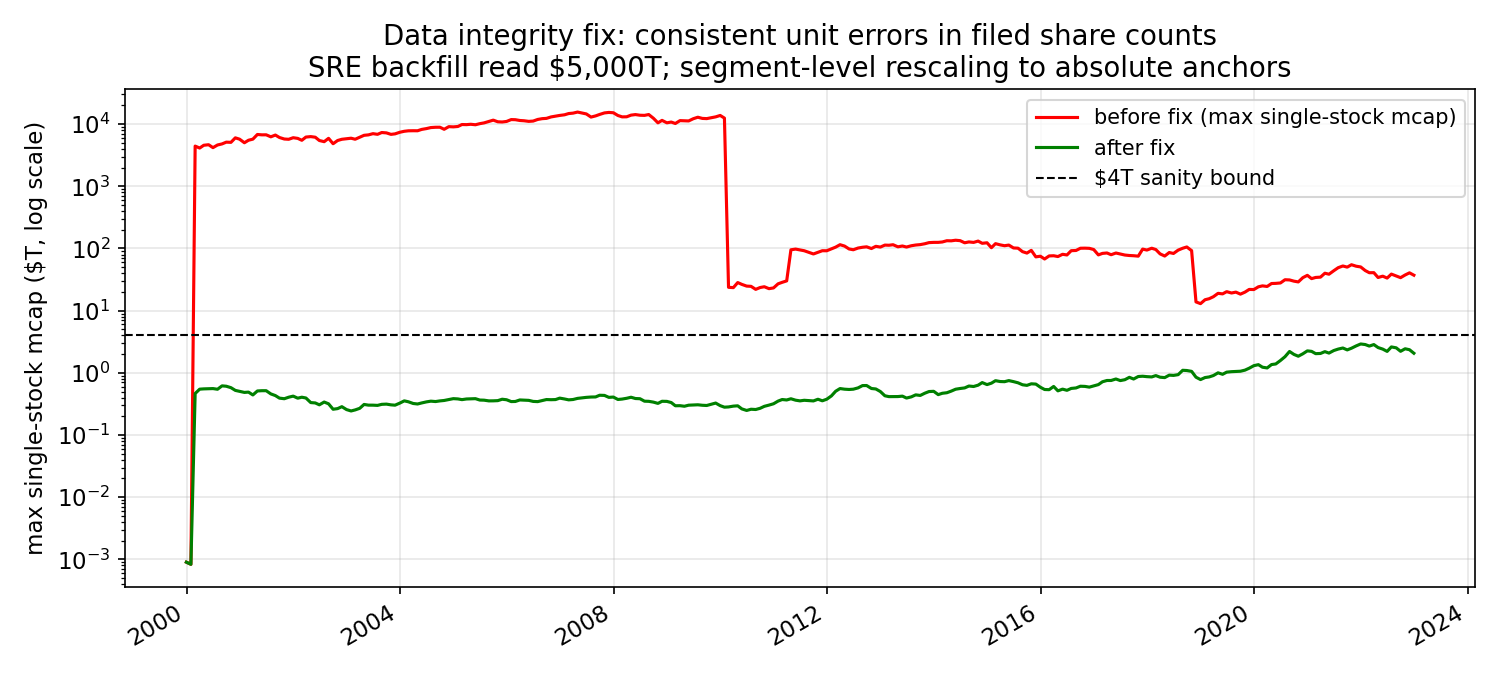
\includegraphics[width=\textwidth]{figures/data_fix.png}
\caption{Data integrity fix: max single-stock market cap before/after segment-level unit rescaling (log scale).}
\label{fig:datafix}
\end{figure}

%=====================================================================
\section{Concentration $\to$ return: pre-registered honest negative}
\label{sec:neg}

Does month-end concentration $C_t$ (top-momentum-lane cap share, \textbf{measured}) predict next-month top-lane excess return over SPY? Two pre-registered forms, estimated 2001--2007 only, judged walk-forward 2008--2022: (1)~threshold-linear $r^e_{t+1} = a + b\max(C_t-0.5,0)$; (2)~quintile means with estimation-window edges. A first run on the pre-fix panel gave a spurious pass driven by the SRE corruption; those numbers are discarded.

Form~1: $b=-0.18$, $t=-0.41$, $R^2=0.002$ (3 months with $C_t>0.5$); walk-forward corr $-0.045$ --- \textbf{fail}. Form~2: Q5$-$Q1 $-0.59\%$/mo in-sample ($t=-0.40$), $-0.52\%$/mo walk-forward ($t=-0.52$) --- meets the letter of the criterion but both spreads are statistically zero, the pattern is non-monotone (in-sample Q5 $+1.23\% >$ Q4 $-0.69\%$), and $\mathrm{corr}(C,r^e)$ is $-0.083$ / $-0.001$. \textbf{Verdict: honest negative.} No $\hat r_b(t{+}1)$ is built; no return portfolio is constructed.

\begin{figure}[t]
\centering
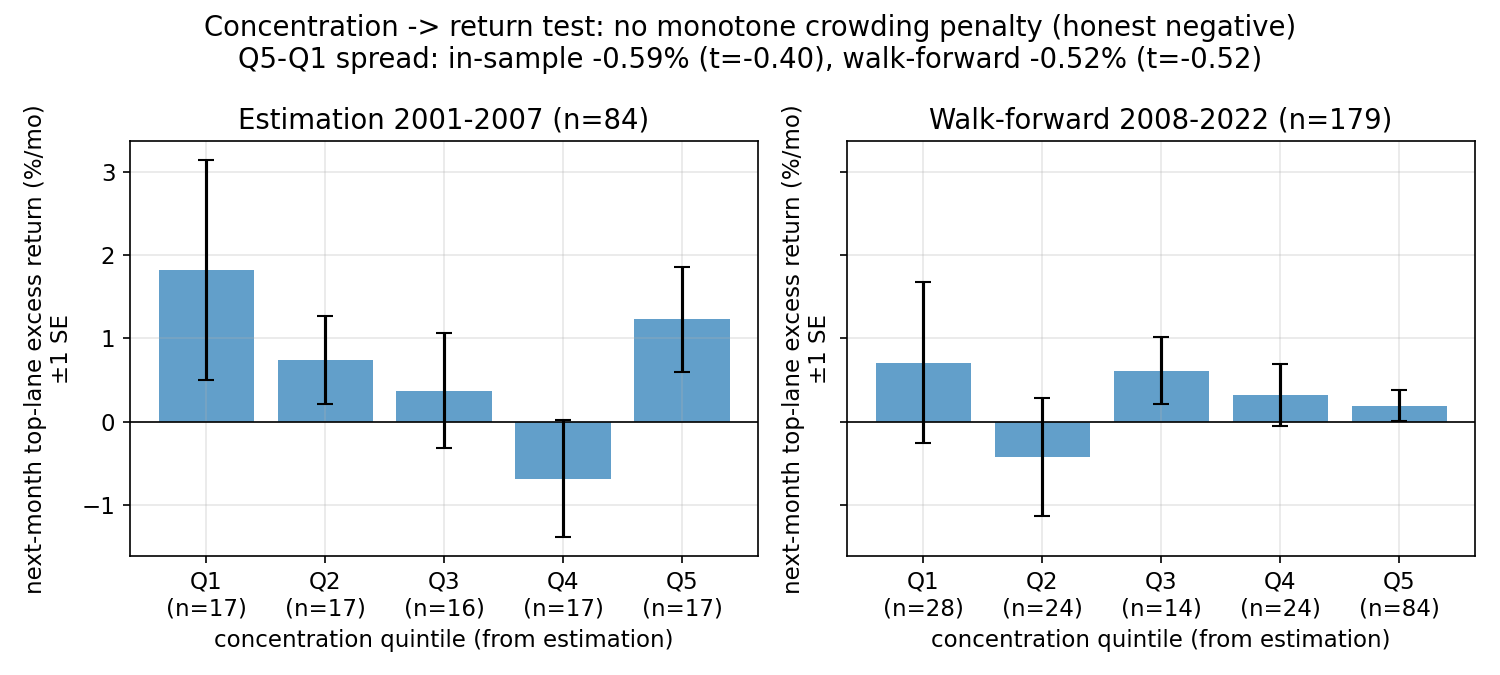
\includegraphics[width=\textwidth]{figures/concentration_test.png}
\caption{Concentration-quintile next-month excess returns, estimation vs.\ walk-forward ($\pm$1 SE). No monotone crowding penalty; error bars swallow every difference.}
\label{fig:ctest}
\end{figure}

%=====================================================================
\section{Risk metrics}
\label{sec:risk}

\subsection{Ensemble distribution forecast with intervals}
The forecastable object remains $\mathbf{c}(t)$. From 2022-12, 200 scenarios: Dirichlet-drawn $T_{\mathrm{calm}}/T_{\mathrm{stress}}$ (mean = measured 2000--2007 $T$; precision = Kish $N_{\mathrm{eff}}$ 109--1825 per bin, \textbf{estimated}; Dirichlet form \textbf{assumed}), AR(1) market driver with bootstrapped residuals (\textbf{estimated}: $a=-0.0006$, $\phi=0.048$), VIX-regime Markov chain (\textbf{measured}), rev-5 calibrated kernels. 12-month-ahead top-lane share: \textbf{median 0.239, 90\% interval [0.106, 0.503]}; HHI [0.110, 0.175]. The intervals are the finding: one-year concentration is dominated by driver and transition uncertainty.

\begin{figure}[t]
\centering
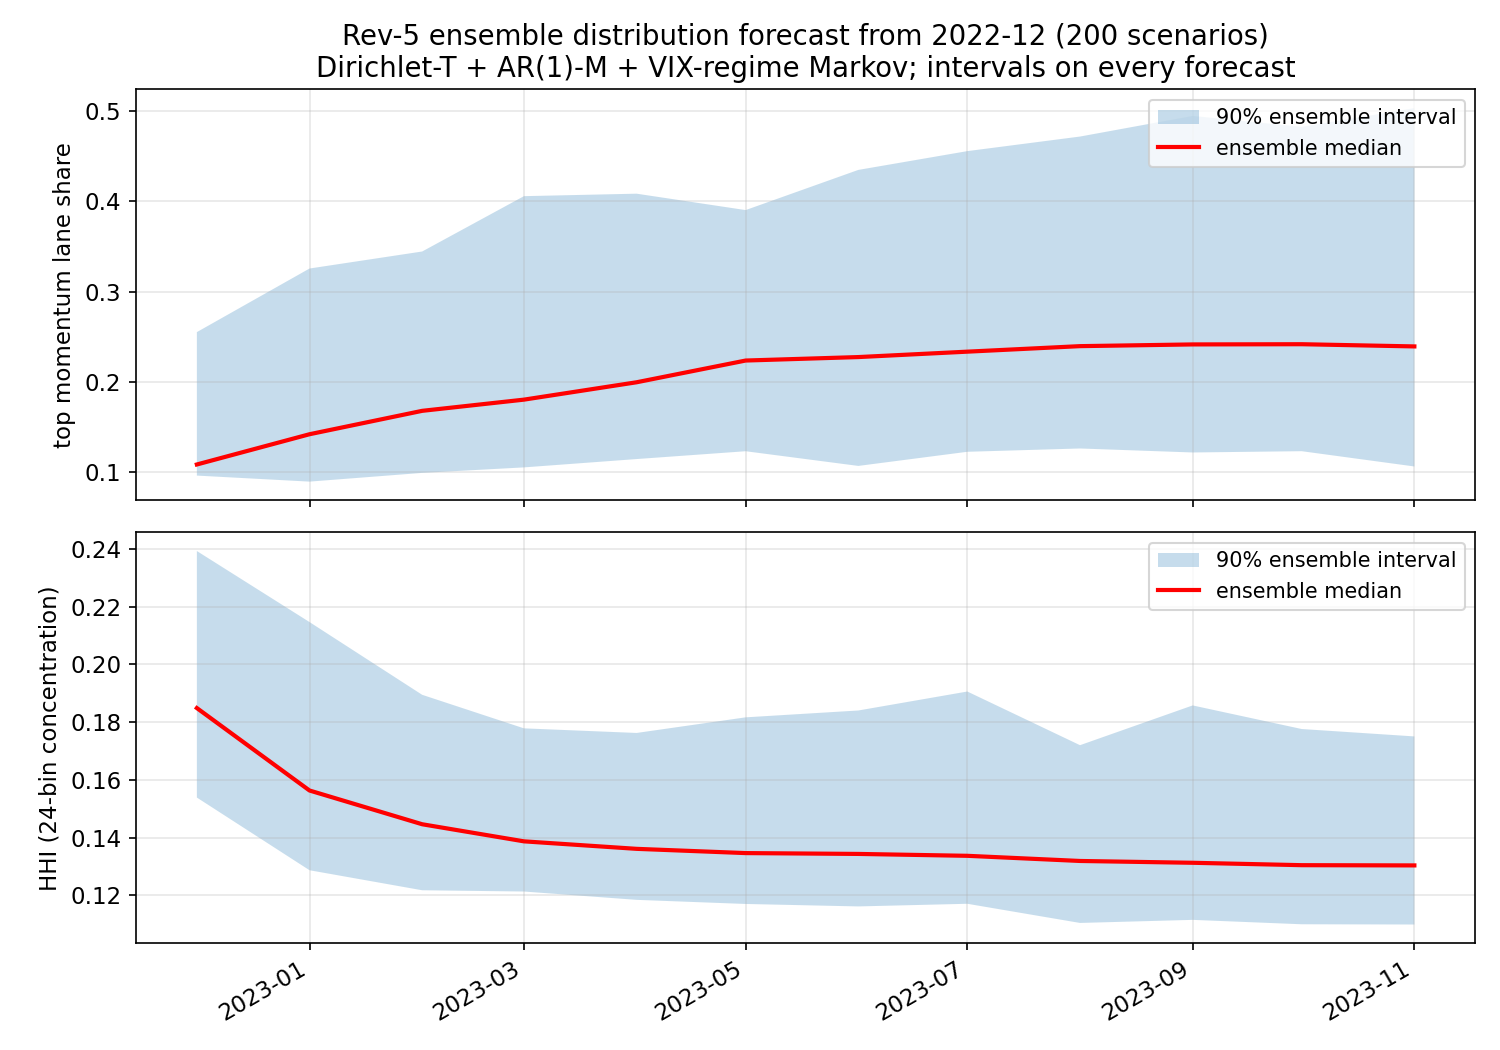
\includegraphics[width=\textwidth]{figures/ensemble_forecast.png}
\caption{Rev-5 ensemble distribution forecast from 2022-12 (200 scenarios): median and 90\% intervals for top-lane share and HHI.}
\label{fig:ens}
\end{figure}

\subsection{Crowding / fragility index}
$C(t)$ and $\mathrm{HHI}(t)$ as percentiles of their own history (full-history diagnostic; expanding-window zero-lookahead). \textbf{Current (2022-12):} $C=0.101$ (25th percentile --- not crowded), HHI $=0.2790$ (52nd). Most crowded: 2004-02 ($0.570$), 2010-01 ($0.571$), 2001-02 ($0.423$). A state descriptor, not a signal (\S\ref{sec:neg}: crowding does not predict returns).

\begin{figure}[t]
\centering
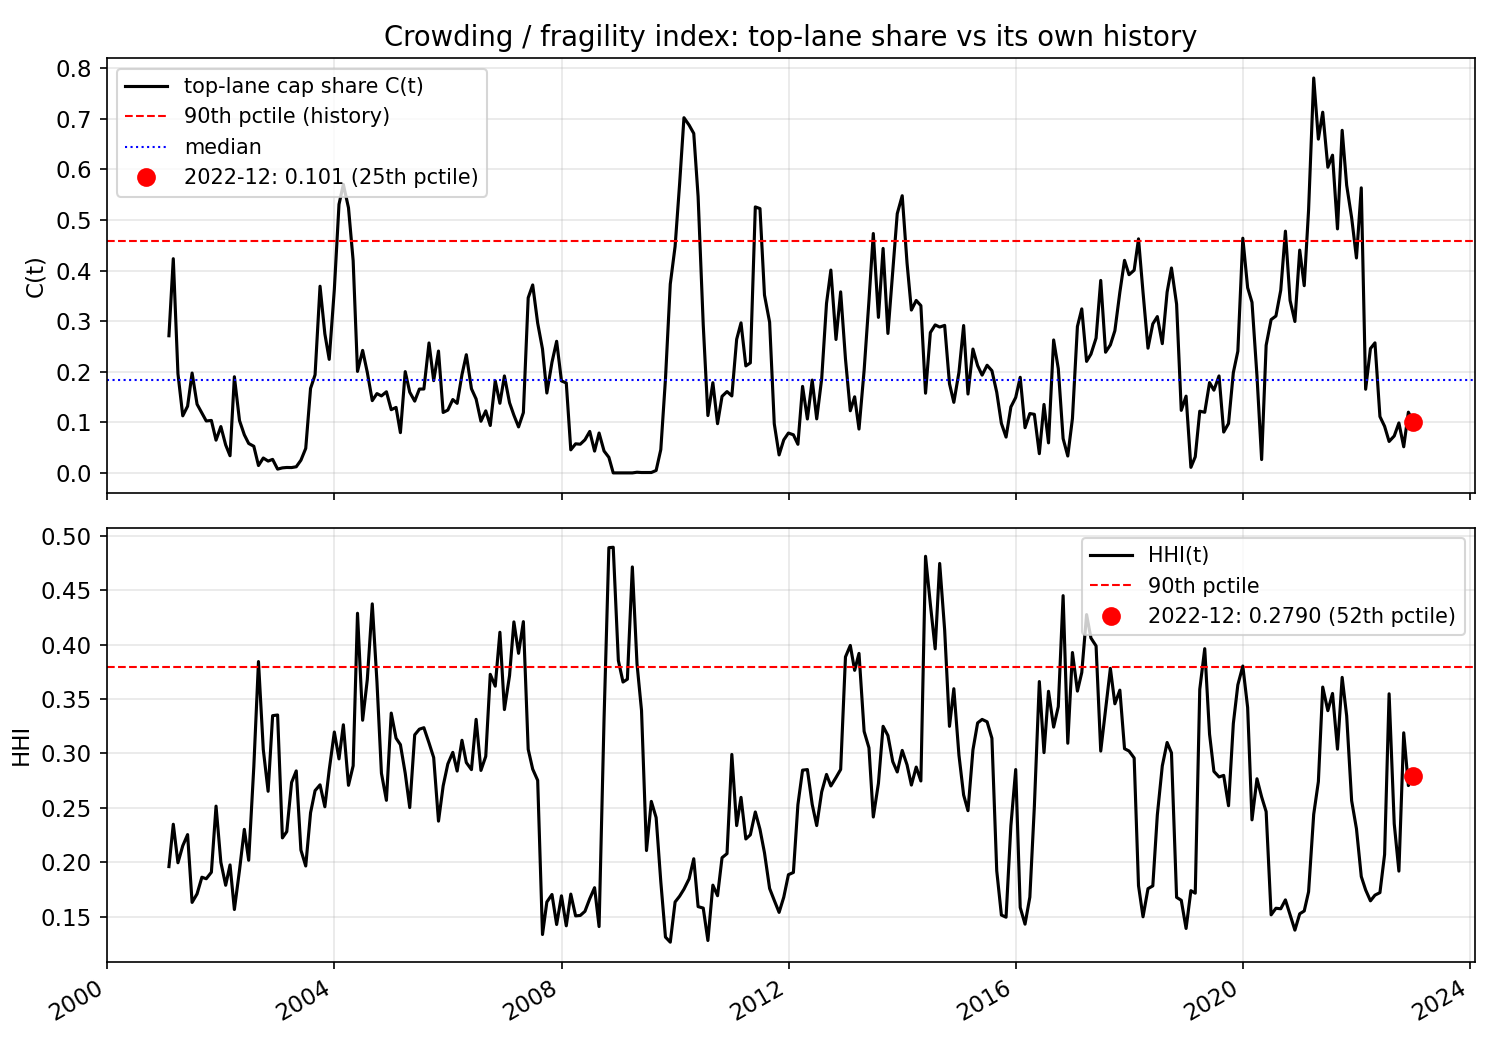
\includegraphics[width=\textwidth]{figures/fragility.png}
\caption{Fragility index: top-lane share and HHI vs.\ own history; 2022-12 readings marked.}
\label{fig:frag}
\end{figure}

\subsection{Portfolio risk}
From the 24-bin return covariance (\textbf{measured}, 2001--2022), the mass-flow tilt (diagnostic only) has predicted annualized volatility \textbf{14.4\%} vs.\ 15.9\% market / 15.4\% SPY realized --- its failure was return-side, not risk-side. Reversal probability $P(\text{top lane trails market next month}\mid C\text{ quintile})$, expanding quintiles: Q1 41.8\%, Q2 44.0\%, Q3 35.8\%, Q4 53.8\%, \textbf{Q5 34.0\%} --- no monotone relationship; the most-crowded quintile reverses least.

%=====================================================================
\section{Re-calibration on clean data}
The 2000--2007 grid re-selects $h_1=0$, $\lambda_1=0$ (clean $T$ plus mechanical advection suffices; $p_{\mathrm{damp}}$ $1.2\to0.8$, still assumed). Clean $T_{\mathrm{calm}}$ differs from rev-4's by up to 0.85 in one transition probability. Conditional hindcasts (realized-$M$ forcing) improve markedly: 2008--09 full RMSE \textbf{0.0899} (was 0.1685; bottom peak 0.83@2009-04 vs.\ 0.99@2009-03); 2020--21 \textbf{0.0714} (was 0.1110; top peak 0.79@2021-04 vs.\ 0.78@2021-03, amplitude exact, one month late).

%=====================================================================
\section{Parameters (rev-5)}
\begin{table}[h]
\centering
\caption{Every input labeled per the standing rule.}
\label{tab:params}
\begin{tabular}{llll}
\toprule
Parameter & Value & Label & Basis \\
\midrule
$h_1$ / $\lambda_1$ & 0 / 0 & calibrated & 2000--2007 grid, clean data \\
Damper $p$/$\tau_{\mathrm{build}}$/gate & 0.8 / 6\,mo / 0.5 & assumed & rev-3 tuning; $p$ re-gridded \\
$T_{\mathrm{calm}},T_{\mathrm{stress}}$ & $24{\times}24$ & measured & cap-weighted, 2000--2007, clean \\
Ensemble & 200 scenarios & assumed & Dirichlet-T + AR(1)-M + VIX-Markov \\
$N_{\mathrm{eff}}$ & 109--1825/bin & estimated & Kish effective transitions \\
$\kappa=1$, $w_{\mathrm{eff}}=0.15$ & --- & mech./assumed & unchanged from rev-4 \\
\bottomrule
\end{tabular}
\end{table}

%=====================================================================
\section{Limitations and next steps}
\begin{enumerate}
\item \textbf{No return model} --- the honest negative is binding: nothing in 2001--2022 supports concentration $\to$ expected returns. Real-capital deployment stays off the table.
\item \textbf{Ensemble is model-conditional} --- intervals cover parameter/driver uncertainty, not misspecification (uniform bins, fixed edges).
\item \textbf{Pre-2009 shares backfilled} (estimated), now unit-fixed; FOX/FOXA/BKR/ETN-backfill dropped.
\item \textbf{Membership} community-sourced~\cite{fja05680}, not official S\&P.
\item \textbf{Form-2 criterion was weak} --- future retests need walk-forward significance, not just sign.
\end{enumerate}

%=====================================================================
\begin{thebibliography}{9}
\bibitem{fja05680} fja05680/sp500. \emph{S\&P 500 Historical Components \& Changes (Updated).csv} --- public GitHub reconstruction; 2,720 snapshots, 1996-01-02--2026-08-18. Point-in-time membership.
\bibitem{yahoo} Yahoo Finance. Daily adjusted closes, corporate-action (split) history, SPY total-return series. Prices, splits, SPY benchmark.
\bibitem{sec} SEC EDGAR. Companyconcept XBRL: \texttt{SharesOutstanding}, \texttt{WeightedAverageNumberOfSharesOutstanding}. Point-in-time shares; \S\ref{sec:datafix} documents the consistent-unit-error repair.
\end{thebibliography}

\end{document}
